\chapter{A keyboard layout for Swahili in Arabic script}
\label{ch:keyboard}

\section{Introduction}

The keyboard layout proposed here is a work-in-progress, and can be adjusted in the light of experience -- I would be happy to receive any suggestions for improvement.  As well as describing the keyboard and explaining the conventions governing the layout, this chapter also includes information on how to edit the layout to suit individual needs.

The \textbf{Andika!} keyboard allows Swahili in Arabic script to be typed directly into a GNU/Linux computer using a standard English (UK or US) keyboard. Input speed is comparable to typing in Roman script.  As well as allowing contemporary Swahili to be easily typed in Arabic script, the keyboard will enable most older manuscripts to be transliterated letter-for-letter.

The complete keyboard layout is depicted in \Cref{fig:kblayout}.\footnote{I am grateful to Wikimedia for the original layout image.} 

\begin{figure}[!ht]
 \centering
 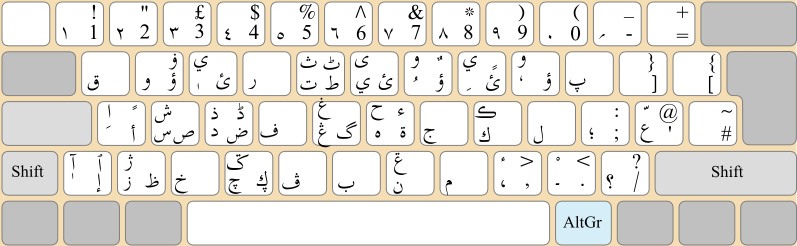
\includegraphics[keepaspectratio=true, scale=0.7]{./images/Swahili_keyboard.png}
 % Swahili_keyboard.png: 797x246 pixel, 90dpi, 22.50x6.94 cm, bb=0 0 638 197
 \caption{Keyboard layout for writing Swahili in Arabic script}
 \label{fig:kblayout}
\end{figure}

As can be seen from Figure \ref{fig:kblayout}, up to four glyphs may be accessed from one key.  To access the contents of each key, the \textbf{Shift} and \textbf{AltGr} keys are used in combination where appropriate, as shown in \Cref{fig:key}.

\begin{figure}[!ht]
 \centering
 \includegraphics[keepaspectratio=true, scale=1]{./images/key.png}
 % key.png: 562x100 pixel, 90dpi, 15.86x2.82 cm, bb=0 0 450 80
 \caption{Accessing the glyphs on the keys}
 \label{fig:key}
\end{figure}

\section{Governing principles for the layout}

The basic governing principle behind the keyboard layout is that the relevant Arabic glyph will usually be produced by pressing the same key that produces the Roman glyph.  It is thus very easy to use: just switch your keyboard to use Arabic script -- in KDE, \textbf{Ctrl+Alt+K} (see \Cref{s:kbactivate} for further information) -- and start typing almost as if the keyboard is being used to type Roman script.  Some examples are given in \Cref{tab:typeeg}.\footnote{For an explanation of the penultimate long vowels accessed by the Shift keys, see \Cref{ch:spelling}.}

\begin{table}[h!]
\centering
\begin{tabularx}{10cm}{rlll}
\textbf{Arabic} & \textbf{Keystrokes} & \textbf{Roman} & \textbf{English}\\
\hline\noalign{\smallskip}
\AS{مِيمِ} & m, i, Shift+i, m, i & mimi & I, me \\
\AS{سَاسَ} & s, a, Shift+a, s, a & sasa & now \\
\AS{لَكِينِ} & l, a, k, i, Shift+i, n, i & lakini & but \\
\AS{نِمٖفِيكَ} & n, i, m, e, f, i, Shift+i, k, a & nimefika & I have arrived \\
\end{tabularx}
\caption{Typing examples}
\label{tab:typeeg}
\end{table}

The other main principle behind the layout is the consistent placement of glyphs that are related by shape or sound in either script:
\begin{itemize}
\item The digraphs \textbf{dh gh th sh zh} are on the same keys as \textbf{d g t s z}, and are accessed using the \textbf{Shift} key.
\item The pharyngeal consonants \AS{ص ض ط ظ} are on the same keys as \textbf{z t d s}, and are accessed using the \textbf{AltGr} key.
\item Similar Arabic glyph shapes are placed on the same key where possible -- for instance \AS{ي ى} are on the \textbf{y} key, and \AS{و ۏ} are on the \textbf{w} key.
\item Long and short vowels are located on the same key, with the long vowel accessed by \textbf{Shift}, so for instance the \textbf{u} key produces \AS{ُ } and \textbf{Shift+u} produces \AS{و}.
\item The vowel carriers \AS{أ إ ئ ؤ} are all accessed using the\textbf{AltGr} key.
\item The alveolar consonants \AS{ٹ ڈ} used in Mombasa Swahili are accessed using the \textbf{AltGr+Shift} keys.
\item The glyphs \AS{و ي} are repeated on \textbf{w y} for use when they represent semi-vowels.
\item The palatal digraph \textbf{ch} is accessed using the \textbf{c} key, and an alternate representation used by some writers, \AS{\char"063B}, is accessed using \textbf{Shift+c}.
\item The occasionally-used digraph \textbf{kh} is accessed using the \textbf{X} key.
\item Non-alphabetic characters from the UK keyboard are currently available via \textbf{AltGr} and \textbf{AltGr+Shift}, in case they might be of use.
\end{itemize}

Further information on the glyphs accessible from each key is available in \Cref{tab:consonants} (consonants) and \Cref{tab:vowels} (vowels).

\section{Changing the layout}
\label{s:changelayout}

The layout of the keyboard is specified in the file \textit{layout/tz}.  Once copied to the appropriate place (see \Cref{s:keyboard}), the layout is available for use.  The file (reproduced in \Cref{appE}) is a simple text file, and can be easily adapted to add new glyphs or change the position of existing glyphs -- see \Cref{appC} for instructions on doing this.

